\documentclass[11pt]{report}
\usepackage{fullpage}
%\usepackage{sourcesanspro, sourcecodepro}
\usepackage{minted}
\usepackage{graphicx}
\usepackage{awesomebox}
\usepackage{hyperref}
\usepackage{float} % stops images from moving around
\usepackage[a4paper, total={6in, 8in}, margin=0.75in]{geometry}
\usepackage{etoolbox}
\makeatletter
\patchcmd{\chapter}{\if@openright\cleardoublepage\else\clearpage\fi}{}{}{}
\RequirePackage[T1]{fontenc}
\RequirePackage[default,light,black]{roboto}

\hypersetup{
    colorlinks=true,
    linkcolor=blue,
    citecolor=blue,
    filecolor=blue,
    urlcolor=blue,
    pdfborder={0 0 0}
}

\graphicspath{{./images/}}

\title{APSC 258: Lab 3 Manual}
\author{Andre Cox}

\begin{document}
\maketitle
\tableofcontents

\clearpage

\chapter{Introduction}
In the previous lab you learnt how to control the PiCar using the Python API. In this lab you will learn how to get video from the PiCar Camera and display it. As well you will also learn how to process the video to make it easier for a neural network to understand. To do this we will use the OpenCV library short for Open Computer Vision. By the end of the lab you should have a processed video stream that can be used to train a neural network. As well you should also gain an understanding of HSV color space.

\chapter{Start of the Lab}
\section{Setup}
On your laptop you will need to install OpenCV you can do this with the following command
\begin{minted}[fontfamily=courier, style=monokai, breaklines, frame=single,framesep=10pt]{shell}
    pip install opencv-python  
\end{minted}

We will use this library to get video from the PiCar Camera. To do this we will write some code.

Try to follow along with the code snippets below to understand how this works. You will need to create a new Python file called imageprocessing.py. We will write the code in this file.

\begin{minted}[linenos, fontfamily=courier, style=monokai, bgcolor=black, breaklines]{python}
    # first we import OpenCV 
    import cv2 as cv 
\end{minted}

Next we will use OpenCV to get video from the PiCar using the built in VideoCapture class.
\begin{minted}[linenos, fontfamily=courier, style=monokai, bgcolor=black, breaklines]{python}
    # we create a variable called ip to store the ip address of the PiCar
    ip = "192.168.0.10"
    # we create a VideoCapture object and tell it to use the ip address of the PiCar
    # as well we use the %s format to insert the ip address into the string
    cap = cv.VideoCapture("http://%s:8080/?action=stream" % ip)
\end{minted}

Now we will use a while loop to get and display the video. If we didn't use a while loop then the video would only be displayed once and then stop.

\begin{minted}[linenos, fontfamily=courier, style=monokai, bgcolor=black, breaklines]{python}
    # we create a while loop to get and display the video
    while True:
        # we get the next frame from the video stored in frame
        # ret is a boolean that tells us if the frame was successfully retrieved
        # ret is short for return
        ret, frame = cap.read()
        # we display the frame
        cv.imshow("PiCar Video", frame)
        # we use the waitKey function to wait for a key press
        # if the key is q then we break out of the loop
        if cv.waitKey(1) & 0xFF == ord('q'):
            break
\end{minted}

Great that was relatively easy. We can connect to the PiCar's WiFi and then run the imageprocessing.py file to get the video. You should see a window open with the PiCar's video streaming to it.

\chapter{Image Processing}
In the last chapter we got the video from the PiCar Camera and displayed it. In this chapter we will learn how to process the video to make it easier for a neural network to understand. To do this we will use OpenCV to isolate the green color from the PiCar's video. As this is the same color of the painters tape we will use to create the track.

\pagebreak

\section{Theory}
Theory is very simple. We will use the HSV color space to isolate the green color. The HSV color space is a color space that is used to represent a color in terms of Hue, Saturation and Value. The Hue is the color and the Saturation is the intensity of the color and the Value is the brightness of the color. You may already be familiar with the RGB color space where Red Green and Blue are mixed with each other to create any color. We use the HSV color space because it is much easier to isolate a range of colors. All we have to do is specify a range of Hue values. 

\begin{figure}[htbp]
    \centering
    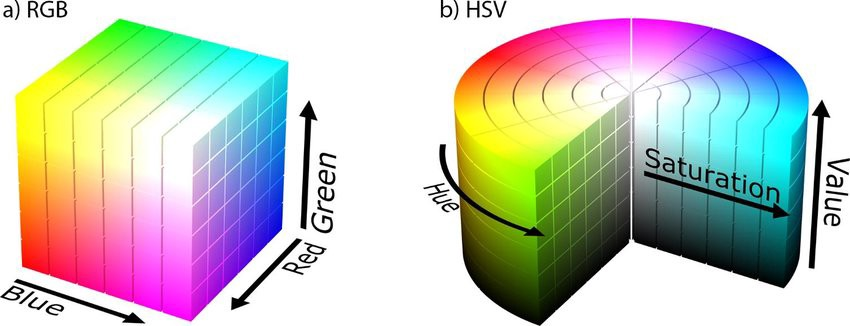
\includegraphics[width=0.8\textwidth]{HSVVSRGB.jpeg}
    \caption{HSV Color Space and RGB Color Space}
    \label{fig:HSVVSRGB}
\end{figure}

From the figure above we can see the RGB color space is a bit confusing. How would we even go about isolating the green color? Isolating in the HSV color space is much easier.

\section{Practice}
Let's practice isolating the green color. To do this we will modify the code we wrote in the previous chapter. Lets add some code to make it find a range of green.

\begin{minted}[linenos, fontfamily=courier, style=monokai, bgcolor=black, breaklines]{python}
    # we create a while loop to get and display the video
    while True:
        # we get the next frame from the video stored in frame
        # ret is a boolean that tells us if the frame was successfully retrieved
        # ret is short for return
        ret, frame = cap.read()
        # we display the frame
        cv.imshow("PiCar Video", frame)

        # now we convert the frame to the HSV color space
        hsv = cv.cvtColor(frame, cv.COLOR_BGR2HSV)

        # I found that these ranges work well for green
        # However you can change the ranges to find other colors
        mask = cv.inRange(hsv, (40, 50, 90), (100, 255, 220))

        # now we display the mask
        cv.imshow("Mask", mask)

        # we use the waitKey function to wait for a key press
        # if the key is q then we break out of the loop
        if cv.waitKey(1) & 0xFF == ord('q'):
            break

\end{minted}

When you run the modified code you should see 2 windows open. The first window is the PiCar's video and the second window is the mask. The mask is a binary image that is black where the green is and white where there is no green. Remember you need to be connected to the PiCar's WiFi to see the PiCar's video.

\notebox{
    \textbf{Reasons for Image Processing:}
    Image processing is used when there is lots of data that could confuse a neural network. This way we can get rid of the data that is not needed. Another upside is that we have just got rid of 1/3 of the data which means the neural network can learn faster.
}

\chapter{End of the Lab}
Now we have a processed video stream that can be used to train a neural network. In the next lab we will train a simple neural network to recognize the track.



\end{document}